\documentclass[openetcs]{template/openetcs_article}
% Use the option "nocc" if the document is not licensed under Creative Commons
%\documentclass[nocc]{template/openetcs_report}
\usepackage{lipsum}
%\usepackage{titledoc}
\usepackage{longtable}
\usepackage{array}
\usepackage{url}
\usepackage{hyperref}
\usepackage{xspace}
\usepackage{graphicx}
\usepackage{supertabular}
\usepackage{fixme}
\usepackage{lscape}
\usepackage{pgfgantt}
\usepackage{adjustbox}
\usepackage{hhline}
\usepackage{booktabs}
\usepackage{multirow}
\usepackage{color, colortbl}
\usepackage[modulo]{lineno}
\definecolor{gray}{rgb}{0.8,0.8,0.8}
\definecolor{myblue}{rgb}{0.6,.6,1}
\definecolor{mydarkblue}{rgb}{0,0,0.5}
\usepackage{datetime}
\graphicspath{{./template/}{.}{./images/}}
\usepackage[color=green!40,textsize=footnotesize,textwidth=2.8cm]{todonotes}
%\usepackage[rond]{natbib}
\graphicspath{{./template/}{.}{./images/}}

\begin{document}


\frontmatter
\project{openETCS}

%Please do not change anything above this line
%============================
% The document metadata is defined below

%assign a report number here
\reportnum{openETCS/WP4/D4.5}

%define your workpackage here
\wp{Work-Package 4: "V\&V Strategy"}

%set a title here
\title{openETCS D4.5: Draft Assessment Report}

%set a subtitle here
\subtitle{Independent Assessment according to the standard EN 50128:2011}

%set the date of the report here
\date{December 2015}


%document approval
%define the name and affiliation of the people involved in the documents approbation here
\creatorname{Fr\'ed\'erique Vall\'ee}
\creatoraffil{All4tec}

\techassessorname{Norbert Sch\"afer}
\techassessoraffil{AEbt}

\qualityassessorname{Marc Behrens}
\qualityassessoraffil{DLR}

\approvalname{Klaus-R\"udiger Hase}
\approvalaffil{DB Netz}


%define a list of authors and their affiliation here
\author{Fr\'ed\'erique Vall\'ee}

\affiliation{All4tec\\
  Immeuble Odyss\'ee B\^{a}timent E \\
  2-12, rue du Chemin des femmes\\
  91 300 MASSY\\
  France\\
 \\
}

\author{Norbert Sch\"afer}

\affiliation{AEbt Angewandte Eisenbahntechnik GmbH\\
  Adam-Klein-Str. 26\\
  90429 N\"urnberg\\
  Germany\\
\\
}





% define the coverart
\coverart[width=350pt]{openETCS_EUPL}

%define the type of report
\reporttype{final version}


\begin{abstract}
The Assessment Report describes the Assessmentresults in the frame of V\&V activities in the openETCS \cite{openETCS} project.
According to the CENELEC EN50128:2011 \cite{EN50128} standard, the assessment is a \"\ Process of analysis to determine whether software, which may include
process, documentation, system, subsystem hardware and/or software components, meets the specified requirements and to form a judgment as to whether the
software is fit for its intended purpose.\"\
\\
\end{abstract}

%=============================
%Do not change the next three lines
\maketitle
%\setcounter{tocdepth}{2}
%\listoffiguresandtables
\newpage
%=============================


% The actual document starts below this line
%=============================


\section*{Modification History}


%\tabletail{}
%\tablelasttail{}





\tablefirsthead{
\hline 
\rowcolor{gray} 
Version & Section & Modification / Description & Author \\\hline}

\bgroup
\def\arraystretch{2.5}%  1 is the default, change whatever you need

\begin{supertabular}{| m{1.2cm} | m{1.2cm} | m{6cm} | m{4cm} |}
 0.1 & all & template of 1st version & Abdelnasir Mohamed \\\hline
 0.2 & all & entering assessment result of ADD document & Fr\'ed\'erique Vall\'ee \\\hline
 0.3 & all & conversion to LaTeX & Marc Behrens \\\hline
\end{supertabular}
\egroup

\tableofcontents
%\listoffiguresandtables
\listoftables

\newpage


\clearpage\section{Information about the Contract}
\subsection{Customer{\textbackslash}
Organization{\textbackslash} Authority}
The customer of the assessment is the OpenETCS project represented by the project leader:

Klaus R\"udiger Hase\\
Project Leader openETCS \\
DB Netz AG\\
Völckerstrasse 5\\
80939 München, GERMANY\\
\\


\bigskip

\subsection{Assessor{\textbackslash}Contractor}
Fr\'ed\'erique Vall\'ee

All4tec\newline
  Immeuble Odyss\'ee B\^{a}timent E \\
  2-12, rue du Chemin des femmes\\
  91 300 MASSY\\
  France\\


\bigskip

Norbert Sch\"afer

AEbt Angewandte Eisenbahntechnik GmbH\newline
  Adam-Klein-Str. 26\\
  90429 N\"urnberg\\
  Germany\\

Recognized independent safety assessor\\
Accredited inspection body DIN ISO/IEC 17020



\bigskip


\bigskip

Contact:

\begin{flushleft}
\tablefirsthead{}
\tablehead{}
\tabletail{}
\tablelasttail{}
\begin{supertabular}{m{4.0020003cm}m{2.3539999cm}m{2.3539999cm}m{7.491cm}}
Norbert Sch\"afer &
~
 &
~
 &
Norbert.Schaefer@aebt.de\newline
+49 911 520992 - 11\\
\\
Fr\'ed\'erique Vall\'ee

~
 &
~
 &
~
 &
Frederique.Vallee@all4tec.net\newline
+33 (0)1 78 85 81 43\\
\end{supertabular}
\end{flushleft}

\bigskip

\clearpage
\bigskip

\subsection{About the contract}

The openETCS organization consists of the openETCS consortium \cite{openETCS} as being initiated by the ITEA2 labelled project \cite{openETCSITEA2}. 

The Assessment is performed on the generic, vendor independent openETCS Software. 
Normally an Assessment for SW and SW development process is done after getting an order from a specific manufacturer{\textbackslash}Producer, 
in this case the customer of the Assessment is the openETCS Consortium itself.

The Safety Integrity Level of the developed SW is SIL4 and therefore an assessment is to be prepared in
accordance with EN 50128:2011 for SIL 4.

Fr\'ed\'erique Vall\'ee (All4tec) and Norbert Sch\"afer (AEbt) have been tasked with the independent assessment of the software and of the software development process of the openETCS.


\bigskip\cleardoublepage
\section{General}
\subsection{Glossary{\textbackslash}List of Abbreviations}
\label{sec:glossary}



\begin{tabular}{rl}
\label{tab:Glossary} 
\textbf{ETCS} & European Train Control System \\ 
\textbf{ERA} & European Railway Agency \\ 
\textbf{EVC} & European Vital Computer \\ 
\textbf{FMEA} & Failure Mode Effect Analysis \\ 
\textbf{SIL} & Safety Integrity Level \\ 
\textbf{SRS} & System Requirement Specification \\ 
\textbf{V\&V} & Verification \& Validation \\ 
\end{tabular}
\captionof{table}{Assessment Glossary}

\bigskip

\bigskip

\subsection{Referenced standards, guidelines and directives}
\bigskip
This document essentially refers to the following standards, ETCS specification documents and openETCS project documents.
%\bigskip

\begin{itemize}
	\item \textbf{ISO~9000} --- 12/2005 --- \emph{Quality management}
	\item \textbf{ISO~9001} --- 12/2008 --- \emph{Quality management systems — Requirements}
	\item \textbf{ISO~25010} --- 03/2011 --- \emph{Systems and software engineering -- Systems and software Quality Requirements and Evaluation (SQuaRE) -- System and software quality models}
	\item \textbf{CENELEC EN~50126-1} --- 01/2000 --- \emph{Railways applications –- The specification and 
		demonstration of Reliability, Availability, Maintenability and Safety (RAMS) –- Part 1: 
		Basic requirements and generic process}
	\item \textbf{CENELEC EN~50128} --- 10/2011 --- \emph{Railway applications -- Communication, signalling and 
		processing systems -- Software for railway control and protection systems}
	\item \textbf{CENELEC EN~50129} --- 05/2003 --- \emph{Railway applications –- Communication, signalling and 
		processing systems –- Safety related electronic systems for signalling}
\item \textbf{CCS~TSI} --- \emph{ CCS TSI for HS and CR transeuropean rail has been adopted by a Commission Decision 2012/88/EU on the 25th January 2012}
\item \textbf{SUBSET-026} 3.3.0 --- \emph{System Requirement Specification}
\item \textbf{SUBSET-091} 3.2.0 --- \emph{Safety Requirements for the Technical Interoperability
	of ETCS in Levels 1 \& 2}
\item \textbf{SUBSET-088} 2.3.0 --- \emph{ETCS Application Levels 1 \& 2 - Safety Analysis}
\item \textbf{OpenETCS FPP} --- \emph{Project Outline Full Project Proposal Annex OpenETCS} -- v2.2
\end{itemize}


\cleardoublepage
\section{Introduction}
\bigskip
\subsection{Initial situation}
\bigskip
The openETCS project has the goal to develop a semi-formal OBU model followed by a strictly formal one realizing functionalities of the UNISIG SRS-SUBSET-026, baseline 3, required for running on the ETCS level 2 of the Utrecht-Amsterdam track. The purpose of this formal model is to increase and spread consistent understanding of the subset, where it can be used as an artifact for testing, analyzing, verification and validation and also for further development pur-poses by industrial actors. This shall be achieved within a framework that is based on an open source concept. The ETCS On Board Unit EVC software model depicted in Figure 1 will be the focus of the software assessment according to the EN 50128:2011.

\begin{figure}
\label{toplevelarchitecture} 
\centering
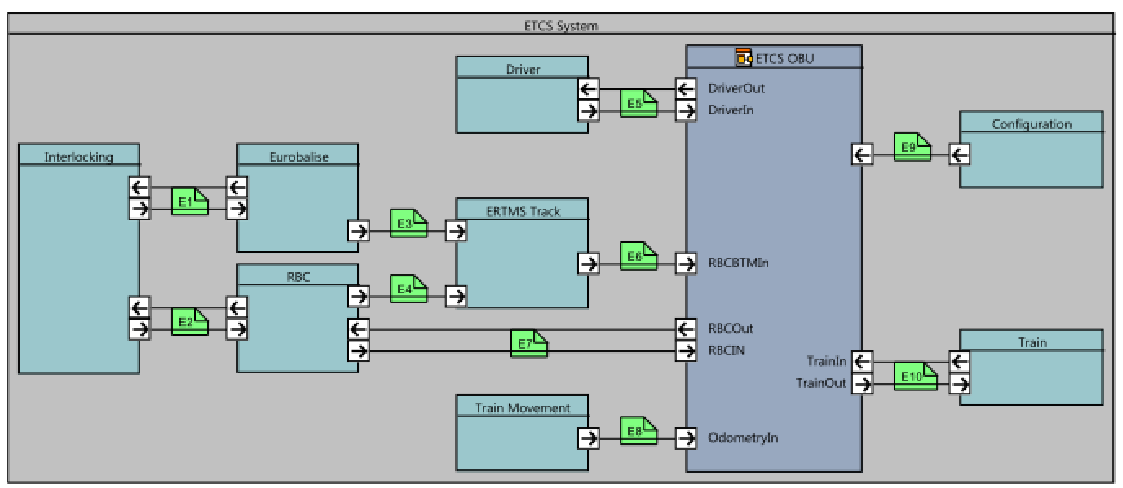
\includegraphics[width=14.552cm,height=6.35cm]{../images/toplevelarchitecture.pdf}
\captionof{figure}{Top level architecture view of the ETCS OBU}
\end{figure}



\bigskip

\subsection{Scope of the assessment}
\bigskip
The scope of the assessment will be the openETCS OBU Software. As it is stated in the Assessment Plan this will cover three main categories:

%\liststyleLiv
\begin{itemize}
\item Project and Software Quality assurance 
\item Verification \& Validation and 
\item Safety 
\end{itemize}

\bigskip

\subsection{Contents of the assessment and issues of concern}
\bigskip
The purpose of this assessment is to answer the following questions relating to software development:

\begin{enumerate}
	\item What measures have been taken to satisfy EN 50128?
	\item Are the measures taken for satisfying EN 50128 SIL 4 sufficient?
	\item Is the agile development practiced in the openETCS project complying with requirements of the EN 50128:2011?
\end{enumerate}
\bigskip

\subsection{Assessment conditions and exceptions}
\bigskip

The ETCS OBU software model has been developed with the closed source SCADE Suite of the company ESTEREL Technology and the code generated is SIL4 certified. Hence only the deliverables of the openETCS software development will have the scope of the
assessment. Also the SoftwareHardware integration is out of the scope of the assessment

\subsection{Documents for the software life cycle and software creation}
\bigskip
The following documents, which describe the software creation process, have been made available to the assessors.


\bigskip

{fixme}% Here i would prefer to add a LaTex Table with only the three columns: 
%1. Documentation (based on EN 50128)
%2. Mapped openETCS (bases on 2.3a Hardis document)
%3. Available openETCS derliverables

\begin{figure}
\label{documentmapping} 
\centering
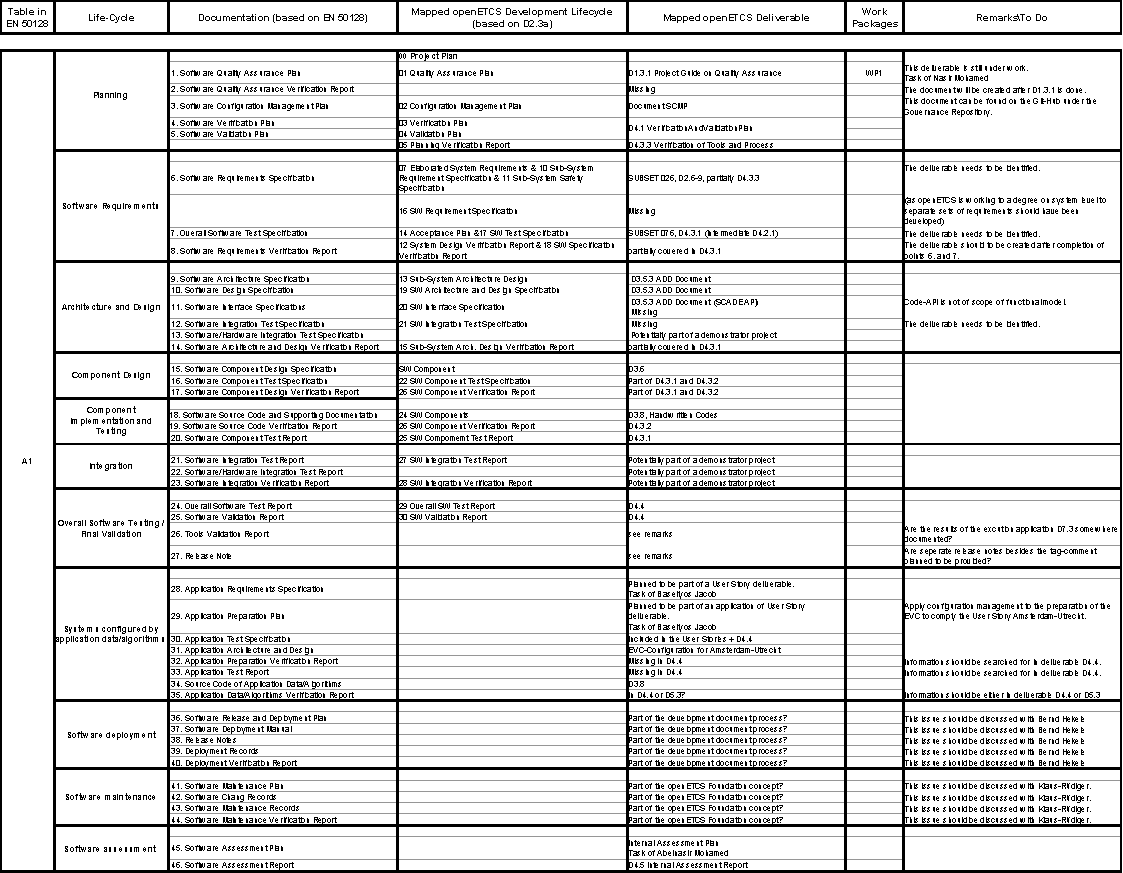
\includegraphics[width=21.001cm,height=16.341cm,angle=-90]{../images/documentmapping.pdf}
\captionof{figure}{Mapping of openETCS Documents to the CENELEC Lifecycle}
\end{figure}



\cleardoublepage
\section{Expert assessment}

\subsection{Process }\label{sec:process-}
\subsubsection{Assessment process}

\bigskip
The openETCS documents from the development process should be made available to the assessor. All documents should be submitted and need to be reviewed for content and form by the assessor as well as reflected and evaluated in the project life cycle and CENELEC standard EN 50128:2011. The results should continually be relayed to the responsible entities within the project Work Packages. Due to the agile workflow in the openETCS project this assessment process should be done iteratively.
\bigskip

\subsubsection{Review of Planning Documents}
The planning documents for quality assurance (software quality assurance plan, software verification plan, software validation plan, software coding standards, software configuration management plan and software maintenance plan) will be reviewed for changes. Also the deliverables will be reviewed for plausibility and compliance with standards.
\bigskip


\bigskip
\subsubsection{Initial Assessment }

As it is stated in the D4.5.1 “Assessment Plan” the assessment process in the openETCS project is performed in an agile way. Following agreed on milestones are listed:

\begin{itemize}	
\item  December 2013 1st assessment
\item  February 2014 1st assessment synchronization meeting Nürnberg
\item  Freeze on project development process assessment related inputs for the assessment: 30.09.2015
\item  Release of Assessment Report part related to project development process assessment related as review: 16.10.2015
\item Freeze on toolchain related inputs for the assessment: 17.10.2015
\item  Release of Assessment Report part related to toolchain as review: 30.10.2015
\item Freeze on documents for assessment: 15.11.2015
\item  Release of Assessment Report as review: 4.12.2015
\end{itemize}


\subsection{Sections assessed}\label{sec:sections-assessed}
The sections of the EN 50128:2011 standard which have been applied for the assessment process on the project are listed in following table.



\tablefirsthead{
	\hline 
	\rowcolor{gray} 
	SECTION TO BE ASSESSED & Section & Was assessed \\\hline}
\begin{supertabular}{| m{6cm} | m{2cm} | m{2cm} |}
	Goals, conformity and software safety integrity level & 4 & yes\\\hline


	 
\end{supertabular} 

\FIXME{\%finishing table from Word document section 4.2}
\bigskip
\bigskip\cleardoublepage
\section{Answers to Questions}

Here a brief description to this chapter (three aspects of Assessment see. AssPlan) 

\subsection{Project Quality Assessment}
\subsubsection{Goals, conformity and SIL [EN 50128 Section 4] PQ}

{\itshape
Goal: allocating the safety related system functions to openETCS SW, as well as SW APIs shall be identified in the
system documentation. Also the SW-SIL shall be specified here. }


\bigskip


\bigskip

Assessment:


\bigskip


\bigskip


\bigskip

\subsubsection{Personnel and responsibility [EN 50128 section 5.1 and 5.2] PQ}
Goal: Ensure that all the staff members are accountable for the software, are organized, competent and capable of
exercising this responsibility.

We have examined the document D1.3.1 ``\textit{Project Quality Assurance Plan''}. 

{\bfseries
ASS512.1}


\bigskip

The openETCS organization consists of seven work packages (WP1 to WP7) where each WP has its own WP-Leader and team
members who shall fulfill the roles and their independency required in the EN 50128:2011. The following image shows the
minimum requirements for the independence of the assessor as well as that between the members of the project team.

 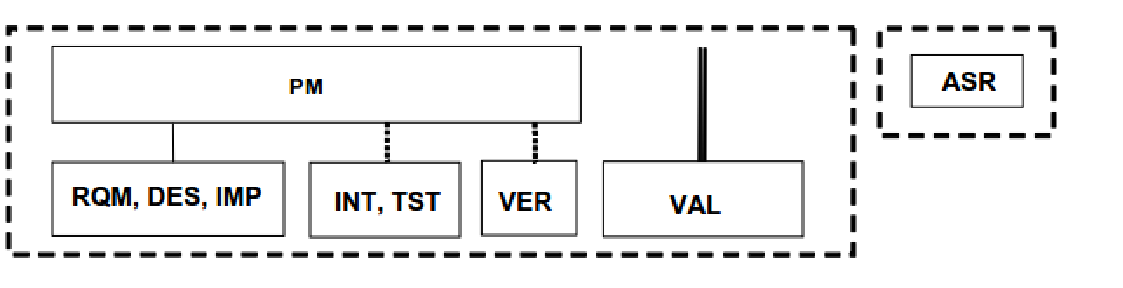
\includegraphics[width=13.626cm,height=3.493cm]{images/organizationalstructure.pdf} 

Figure 2: Preferred organizational structure for SIL 4 SW-Development

WP-Leader 1 (WPL1) is the project manager of the whole project. For the actual development three WPLs have an equivalent
role to that of a project manager depicted in Figure 1. Other roles are distributed within the different WPs depending
on their tasks and goals.


\bigskip

\begin{center}
\tablefirsthead{}
\tablehead{}
\tabletail{}
\tablelasttail{}
\begin{supertabular}{|m{5.467cm}|m{5.467cm}|m{3.467cm}|}
\hline
EN 50128:2011 Role  &
Person  &
WP (Entity) \\\hline
Project manager of all WPs  &
Mr. Dr. Hase (DB)  &
WP1 \\\hline
WPLs as Project manager  &
Mr. Cochetti (Alstom)  &
WP3\\\hline
~
 &
Mr. Behrens (DLR) &
WP4\\\hline
~
 &
Mr. Deutsch (ERSA)  &
WP5\\\hline
~
 &
Mr. Jastram (Formal Mind)  &
WP7\\\hline
\end{supertabular}
\end{center}
Table 1 Work package Leaders as project manager


\bigskip

Assessment:

For the targeted SIL4 the roles were chosen appropriately within the openETCS organization. There are seven WPLs where
the WPL1 is also the leader of all WPLs. The Assessors have examined the independencies of the roles within the
openETCS organization and came to following conclusions:

{}-- Although the validator belongs organizationally to WP4 he is an independent entity in the openETCS project and does
not underlie the WPL1, WPL3, WPL5 neither WPL7.

{}-- The verifiers are not the same persons as the entities integrator, Tester, requirements manager, designer nor
implementer

{}-- The independency of the rest of the entities is guaranteed according to Figure 1.

Due to the fact that every project partner is EN ISO 90001 certified in addition to the many technical discussions the
assessors had held with the WPLs or the many attended openETCS Scrum meetings the assessors can confirm the competences
of the WPLs and their team, which are listed in the competence matrix in the QAP.

The training and qualification of the project participants is also sufficient for the tasks to be implemented. For
example a SCADE Suite training is held for all partners using the SCADE Suite software tool in 2014.

This requirement is fulfilled.

\subsubsection[5.1.3 Life cycle and documentation [EN 50128 section 5.3{]} PQ]{5.1.3 Life cycle and documentation [EN
50128 section 5.3] PQ}
Goal: Organization of the software development into set phases and activities as well as registration of all the
information used for the software throughout the entire life cycle of the software.

Assessment:


\bigskip


\bigskip


\bigskip

\subsubsection[5.1.4 Software quality assurance [EN 50128 section 6.5{]}* PQ]{5.1.4 Software quality assurance [EN 50128
section 6.5]* PQ}
(*): other EN 5018 parts to be examined here = \textit{sections 7.3.4.25 to 7.3.4.27 related to coding standards. }

Goal: Identification, monitoring and controlling of all technical and management activities that are necessary in order
to ensure that the software attains the required quality. This is necessary to guarantee the required qualitative
defense against systematic faults and to ensure that an audit can be set up to make it possible to efficiently take
verification and validation measures. 


\bigskip

Assessment:


\bigskip

The description of the process of configuration management (above list) is not described in enough detail and is to be
improved.


\bigskip

\subsubsection{Changes and change management [EN 50128 sect. 6.6] PQ}
Goal: Ensure that the software functions as required and that the software safety requirement and reliability is
retained upon modification of the software.


\bigskip

Assessment:


\bigskip

\subsection{V\&V Assessment}

\bigskip

\subsubsection{Software test [EN 50128 sect. 6.1]* V\&V}
(*): other EN 5018 parts to be examined here = section 7.3.4.33 (software component test specification) and sections
7.3.4.29 to 7.3.4.40 (software integration and software/hardware integration specifications)

The goal of the software test is to check the behavior or performance of the software.


\bigskip

Assessment:

\subsubsection{Software verification [EN 50128 sect.
6.2]* V\&V}
(*): other EN 5018 parts to be examined here = sections 7.3.4.41 to 7.3.4.43 (software architecture and design
verification).


\bigskip

The goal of the software verification is the investigation and evaluation based on demonstrating that the results of a
certain development phase are sufficient.

Assessment:


\bigskip

\subsubsection[5.2.3 Software validation [EN 50128 sect. 6.3{]} V\&V]{5.2.3 Software validation [EN 50128 sect. 6.3]
V\&V}
The goal of the software validation is to demonstrate that the processes and output variables of the software comply
with the set SIL, satisfy the software requirements and are suitable for the intended application. The main validation
activities consist of analysis and/or testing and evaluation of the safety criticality of all the faults and
deficiencies.


\bigskip

Assessment:


\bigskip

\subsubsection{Software implementation and test
(EN 50128 sect. 7.5) V\&V}
Goal: Creation of software that is analyzable, testable, verifiable and repairable. This phase also covers component
tests.


\bigskip


\bigskip

Assessment:


\bigskip


\bigskip

\subsubsection{Software integration (EN 50128 sect. 7.6) V\&V}
Goal: Execution of the software integration and software/hardware integration. Demonstration that the software and the
hardware properly work together to perform their intended functions.


\bigskip


\bigskip

Assessment:


\bigskip

\subsection{Safety Activities Assessment}

\bigskip

\subsubsection{Software assessment [EN 50128 sect. 6.4] SA}
Goal: Evaluation of the process of the life cycle and the products arising from it allow the conclusion that the
software exhibits the set SIL 1 to 4 and is suitable for it intended use.


\bigskip

Assessment:


\bigskip

\subsubsection{Supporting tools and languages [EN 50128 sect. 6.7] SA}
Goal: Software tools must be appropriately selected for the software development process, the tools should be able to
work together, the use of tools in classes T2 and T3 must be justified and for T3 proof of suitability must be present.


\bigskip


\bigskip

Assessment:


\bigskip

\subsubsection{Software requirement (EN 50128 sect. 7.2) SA}
Goal: Description of a complete set of requirements for the software that satisfies all the system and safety
requirements and provides an extensive set of documents for each later phase.


\bigskip


\bigskip


\bigskip

Assessment:


\bigskip

\subsubsection{Software architecture and design
(EN 50128 sect. 7.3) SA}
Goal: Development of a software architecture. Identify and evaluate what the interaction between hardware and software
means for safety. Selection of a design process. Design of the software of a defined SIL. Ensure that the resulting
system and its software can easily be tested from the outset.

We have examined the document: D3.5.3 ``openETCS Architecture and Design Specification''.

Notice that the section 7.3 of EN 50128 covers not only architecture, interface and design specifications but also test
specification for software component test, software integration and software/hardware integration. These elements are
not covered by D3.5.3. So section 7.3.4.33 and sections 7.3.4.29 to 7.3.4.40 have been transferred to \& 5.2.1 of this
document. For the same reason, sections 7.3.4.41 to 7.3.4.43 dealing with verification have been transferred to \& 5.2.2
of this document, and sections 7.3.4.25 to 7.3.4.27 related to coding standards have been transferred to \& 5.1.4 of
this document.

{\bfseries
ASS534.1}

Considering the safety aspects we have some doubt about the robustness of the proposed design. Theoretically the
following fields ``Behaviour when value is at boundary / Behaviour for values out of valid range / Behaviour when value
is erroneous, absent or unwanted'', given for all inputs should explain which safety mechanisms have been implemented
and how they work . Numerous remarks can be done on these fields:

{\textbullet} Sometimes the behavior in case of ``erroneous data'' is considered as identical to the behavior in case of
``data at the boundary'' which is not acceptable (see for example 5.2.2.1.3 ActualOdometry; 5.2.2.1.11
inSupervisingRbcId {\dots}).

{\textbullet} Sometimes the behavior in case of ``erroneous data'' could result in a hazard but no safety mechanism is
proposed (see for example 5.2.2.1.13 q\_nvlocacc; 5.3.2.1.2 Status\_MA\_FS\_SR\_OS\_LS\_SH\_from\_MA\_L2\_Management;
5.3.2.1.8 statusValid\_Position\_from\_Position\_Calculation {\dots}).

{\textbullet} A majority of these fields indicates ``n/a'' and that seems very curious for a SIL4 software. These n/a
should be justified (For example, the input ``5.9.2.1.19 SafetyCriticalFailure'' is considered has having no effect
when it is absent or erroneous which is very curious considering the name of the data).


\bigskip

{\bfseries
ASS534.2}

Requirement 7.3.4.5 of the EN 50128 is: ``The Software Architecture Specification shall identify, \textbf{analyse and
detail the significance} of all hardware/software interactions''. This requirement is not fulfilled.


\bigskip

{\bfseries
ASS534.3}

Requirement 7.3.4.6 b) of the EN 50128 is: ``Software components shall be clearly identified and \textbf{independently
versioned inside the configuration management system}{}''. This requirement is not fulfilled.


\bigskip

{\bfseries
ASS534.4}

The following EN 50128 requirements are not fulfilled:

{\textbullet} 7.3.4.10 The Software Architecture Specification shall \textbf{describe the strategy for the software
development} to the extent required by the software safety integrity level. 

{\textbullet} 7.3.4.11 \textbf{Measures for handling faults} shall be included in the Software Architecture
Specification in order to achieve the balance between the fault avoidance and fault handling strategies.


\bigskip

{\bfseries
ASS534.5}

The Software Interface Specification (see requirements 7.3.4.18 and 7.3.4.19 of EN 50128) is missing. The description of
interface data given in D3.5.3 is incomplete [a) pre/post conditions; f) allocated memory, f) and h) synchronization
mechanisms are missing].


\bigskip

{\bfseries
ASS534.6}

The description given in the software design part does address neither the main algorithms and sequencing or concurrency
aspects, nor the error reporting mechanisms (see f) and g) of requirement 7.3.4.23 of EN 50128 and b3) and b4) of
requirement 7.3.4.28 of EN 50128. 


\bigskip

Assessment:

Design Specification is incomplete (Scrum process) but numerous requirements of the CENELEC standard are not fulfilled
and will not be if the content of the document is not modified. 

Notwithstanding these previous remarks, a major remark is that safety aspects are not well addressed in this design.

\subsubsection{Software components design (EN 50128
sect. 7.4) SA}
Goal: development of a software component design and software component test specifications, with which the requirements
of the software design specifications are satisfied to the extent required by the SIL.


\bigskip


\bigskip

Assessment:


\bigskip


\bigskip

\subsubsection[5.3.6 Overall software test [EN 50128 sect. 7.7{]} SA]{5.3.6 Overall software test [EN 50128 sect. 7.7]
SA}
Analysis and test of the integrated SW and HW in order to ensure accordance with the software requirement
specifications, especially the functional and safety aspects as per the SIL.


\bigskip

Assessment:


\bigskip

\subsubsection{Application data or algorithms -- systems configured by application data or algorithms [EN 50128
sect. 8] SA}

\bigskip


\bigskip


\bigskip

Assessment:


\bigskip


\bigskip

\subsubsection{Deployment of the software [EN 50128
sect. 9.1] SA}
Goal: Ensure that the software works as intended, adheres to the required SIL and reliability when it is deployed in the
final environment of application


\bigskip


\bigskip

Assessment:


\bigskip


\bigskip

\subsubsection{Maintenance of the software [EN 50128 sect. 9.2] PQ or SA}
Goal: Verification that the software functions as required and the obligatory SIL and reliability are maintained if
corrections, extensions or adjustments are performed on the software.


\bigskip


\bigskip

Assessment:


\bigskip

\subsection{Answer to the question: \newline
Are the measures taken for satisfying EN 50128 SIL 4 sufficient?}
Answer to the above question

\subsection{5.5 OTHER Question?}
{\textbullet} E.g.: Agile development in openETCS and its conformity to the EN 50128 

{\textbullet} {\dots}.\cleardoublepage
\section{Summary}

\bigskip
The assessors were charged by the openETCS project management board to assess the process of the software development of the openETCS according to the EN 50128:2011.

The main outcomes of the project are the openETCS software and the openETCS tool chain. A high degree of standardization of a vital part of the ETCS System Requirement Specifica-tion prose (normal textual language) was reached by applying the formal methods (FM) con-cept. This has been resulting in a functional interpretation of the ETCS software. For a SIL level 4 software development the EN 50128:2011 has classified the Formal Methods as “Highly Recommended” as for the techniques/measures to
\begin{itemize}
\item	software requirements specification,
\item	software architecture,
\item	software design and implementation,
\item	verification and testing.
\end{itemize}

Since the openETCS toolchain software lacks the maturity for industrial use and the con-straints the standard EN 50128:2011 entails, the PMB has decided to pursue the openETCS SW development with the closed source Tool SCADE Systems and SCADE Suite. This has led to major progress towards developing the ETCS software with the FM approach.

Still the developed software does not cover all the ETCS requirement specifications. The quality of the software development process is not sufficient for the required safety integrity level. A lot of work still needs to be done to fulfill the CENELEC standard to a 100\% in the area of the development process.
\cleardoublepage
\section{Tasks, recommendations and notes}

\bigskip

This sections describes the recommendations for a follow-up assessment when incorporating openETCS results.\cleardoublepage
\section{Finalization}



\begin{flushleft}
\tablefirsthead{}
\tablehead{}
\tabletail{}
\tablelasttail{}
\begin{supertabular}{| m{17cm}} 
\\
Nuremberg, \\
~

~

~
\\
~
\\
\\
Expert assessor\\

Norbert Sch\"afer\\
~
\\
\\
\\
\\
\\

Massy, \\
~

~

~
\\
~
\\
\\
\\
\\
Expert assessor\\

Fr\'ed\'erique Vall\'ee\\
\end{supertabular}
\end{flushleft}

\bigskip


\bigskip



\bigskip
\cleardoublepage

% show only documents cited
%\nocite{*} 

\bibliographystyle{plain}
\bibliography{ref/Assessment_Report}



%===================================================
%Do NOT change anything below this line

\end{document}
